\section{Модель монополии профсоюза на временных шкалах}

В игре, как и в непрерывной модели присутствует два игрока: профсоюз $P$ и фирма $F$, чьими рычагами влияния на игру являются $W$ - зарплата рабочего и $E$ - количество нанятых рабочих соответственно.
Каждый игрок выбирает из следующих стратегий: низким $L$ и высоким $H$ уровнем повышения. В общем виде игра может быть задана следующей матрицей выигрышей: 

\begin{table}[h]
	\centering
	\begin{tabular}{|l|l|l|l|}
		\hline
		\multicolumn{2}{|l|}{\multirow{2}{*}{}} & \multicolumn{2}{l|}{Профсоюз} \\ \cline{3-4} 
		\multicolumn{2}{|l|}{}                  & $L$            & $H$            \\ \hline
		\multirow{2}{*}{Фирма}     & $L$     & $a,q$          & $b,v$          \\ \cline{2-4} 
		& $H$     & $c,x$          & $d,z$          \\ \hline
	\end{tabular}
\end{table}
Функция полезности профсоюза  $U_t(W,E)=\lambda WE$, где $\lambda \in(0;1)$:
$$\frac{\partial U}{\partial W} > 0; \quad \frac{\partial U}{\partial E}~>~0 \quad U(0,E)=U(W,0)=U(0,0)=0,$$


Функция полезности фирмы $\Pi_t(W,E)=cP(\bar{K},E)-WE$:
$$P(\bar{K}, E)=A\bar{K}^\alpha E^\beta,$$ где $A$ – коэффициент нейтрального технического прогресса, $\alpha$ и $\beta$ – коэффициенты эластичности валового внутреннего продукта по капитальным и трудовым затратам.\\

Для профсюза соотношения функции полезности для всех стратегий будет следующим:
\begin{equation}
U(L,L) < U(L,H) \thickapprox U(H, L) < U(H,H),
\end{equation}
где соотношение $U(L,H) \thickapprox U(H, L)$ неопределенное, так как это чисто "политический" момент, что для профсоюза более выгодно: большее количество людей, получающих меньшую зарплату или меньшее количество людей, получающих большую зарплату. 

Для нахождения соотношений между функциями полезности для фирмы построим график~\ref{fig:monopoly_union1}.\\

\begin{figure}[h]
	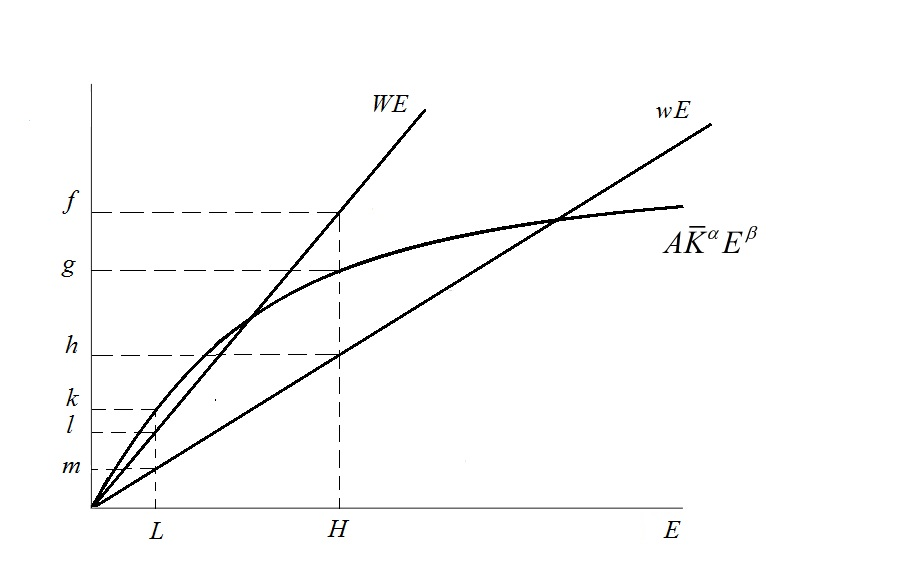
\includegraphics[width=1.0\linewidth]{monopoly_union2.jpg}
	\caption{}
	\label{fig:monopoly_union1}
\end{figure}
где $w$ - низкий уровень зарплат по стратегии $L$, а $W$ - высокий уровень зарплат по стратегии $H$. 
Принимая во внимание, что все коэффициенты константы за исключением количества нанятых и уровня зарплат, легко вывести следующее:
 
\begin{equation}
\Pi(H,H)=g-f < \Pi(H,L)=k-l < \Pi(L, L)=k-m < \Pi(L,H)=g-h.
\end{equation}
Следовательно матрица выигрышей будет следующей:
\begin{table}[h]
	
	\centering
	\begin{tabular}{|l|l|l|l|}
		\hline
		\multicolumn{2}{|l|}{\multirow{2}{*}{}} & \multicolumn{2}{l|}{Профсоюз} \\ \cline{3-4} 
		\multicolumn{2}{|l|}{}                  & $L$            & $H$            \\ \hline
		\multirow{2}{*}{Фирма}     & $L$     & $a,q$          & $b,v$          \\ \cline{2-4} 
		& $H$     & $c,x$          & $d,z$          \\ \hline
	\end{tabular}
		\caption{}
			\label{table:firm}
				
		
\end{table}\\
где $q < x \thickapprox v < z, 0 > d < b < a < c$
